\documentclass[10pt]{article}

\usepackage{amssymb, amsmath, lineno, enumitem, float, epstopdf, graphicx}
\usepackage[margin=1in]{geometry}
\title{Genealogical Properties under the Moran Model}\author{Arjun Biddanda}
\date{\today}
% Removes the page numbering
\pagenumbering{gobble}

\begin{document}
\maketitle
% \linenumbers

\section{Definitions and Notation}

There are many definitions for the Moran Model, but we will adopt the model according to the following algorithm:

\begin{enumerate}
	\item Choose one individual to ``die''
	\item Choose one individual (it may be the same individual) to reproduce and have 2 offspring
\end{enumerate}

Note that this differs considerably from the aspects of the Discrete-Time Wright-Fisher (DTWF) model in that by construction multiple-mergers are not allowed to occur within a generation. However, all of the other relevant genealogical properties are available.

\section{Appendix and Notes}

\subsection{Initial Derivations}

\subsubsection{Probability of Lineage Reduction}
Initially we want to derive the probability that the number of lineages is reduced from $n$ to $m$ from the $t^{\text{th}}$ to the $(t+1)^{\text{th}}$ generation :

$$
\begin{aligned}
	p^{(t)}_{n,n-1} &= \frac{n}{N_{t+1}}\cdot \frac{(n-1)}{N_{t+1}}\\
	&= \frac{n(n-1)}{N^2_{t+1}}\\
	p^{(t)}_{n,n} &= 1 - p^{(t)}_{n,m}\\
	&= 1 - \frac{n(n-1)}{N^2_{t+1}}\\
\end{aligned}
$$

We can compactly represent this function as:

\begin{equation*}
	p^{(t)}_{n,m} = 
	\begin{cases} 1 - \frac{n(n-1)}{N^2_{t+1}}  & \text{if $m = n$,}
		\\
		\frac{n(n-1)}{N^2_{t+1}} &\text{if $ m = (n-1)$,}
		\\
		0 &\text{else.}
	\end{cases}
\end{equation*}

We note that as $t$ is increasing, we are moving farther back in time (e.g. the ($t+1)^{th}$ generation is gene generation immediately before the $t^{th}$. The rationale for the derivation is that in order to reduce the number of lineages by 1, we must pick one of $n$ individuals to then be ``replaced'' by one of $n-1$ individuals. 

This is a very simplistic representation of the Moran model and can be extended to support a higher birth rate (which can potentially yield multiple mergers). We plan to discuss these more general forms in greater detail towards the end of the analysis. 

We can then extend this to $p^{(t')}_{n,m}$, or the probability that $n$ samples in generation $t$ have $m$  ancestors in generation $t'$. Due to the construction of the Moran Model, we are required to bound the quantity $m$ such that $n-t' \leq m \leq n$, otherwise the probability is $0$. Thus we obtain the following recursion :

$$
\begin{aligned}
	p^{(t, t')}_{n,m} &= \Bigg[\frac{n(n-1)}{N_{t+1}}\Bigg] p^{(t, t'-1)}_{n-1, m} + \Bigg[1 - \frac{n(n-1)}{N_{t+1}}\Bigg] p^{(t, t'-1)}_{n,m}\\
	p^{(t, t)}_{n,n} &= 1\\
\end{aligned}
$$

The recursion holds when $t' \geq t$. Having this recursion relation allows us to look at lengths of time that are longer than just a single generation. This allows us to look at the long range time-scaling of the process that is needed to compare the Moran Model to the coalescent. 

We would expect that when the sample size gets larger, the proportion of lineages that are lost successively in the generations of the Moran model will be quite a bit higher. 

\subsubsection{Expected Number of Lineages as a Function of Time (NLFT) under the Moran Model}

Now that we have the following we can think of time $t$ in much larger steps (e.g. in increments of $t_{scaled}$) such that we can now define the probability of having $m$ ancestral lineages (conditional on $n$ lineages at time $t = 0$. These results directly mirror those of Bhaskar et al, but now with the recursion derived for the Moran Model:

 \begin{equation*}
	 \mathbb{P}[A^M_n(t) = m] =
	 \begin{cases} 
		 \sum^n_{k=m}  p^{(t-t_{scaled}, t)}_{k,m} \mathbb{P}[A^M_n (t-t_{scaled}) = k],  &\text{if $t > 0$,}
	 	 \\
		 \delta_{n,m} &\text{if $t = 0$}
	 \end{cases}
 \end{equation*}

 Where $\delta$ takes a value of $1$ when $n=m$ and $0$ elsewhere. From this realization, we can directly calculate the NLFT in the Moran Model as:

 \begin{equation*}
	 \mathbb{E}[A^M_n(t)] = \sum^n_{m=1} m \mathbb{P}[A^M_n (t) = m]
 \end{equation*}

\subsubsection{Sample Frequency Spectrum under the Moran Model}

We would also like to obtain the expected Site Frequency Spectrum (SFS) under the Moran Model. We will use the same notation and general derivation as Bhaskar et al.

We set the entry $\tau_{n,k}$ as the number of sites at which $k$ individuals carry the derived allele and $n-k$ individuals carry the ancestral allele. Thus we can then define the entire SFS as $\tau_n = (\tau_{n,1}, ..., \tau_{n,n-1})$. 

We will further define $\gamma^{(t)}_{a,b}$ as a random variable representing the total branch length of a subtree that subtends a set of $a$ individuals in a larger set of $a+b$ individuals. 




\newpage

\subsection{Preliminary Figures}

\begin{center}
\begin{figure}[!h]
	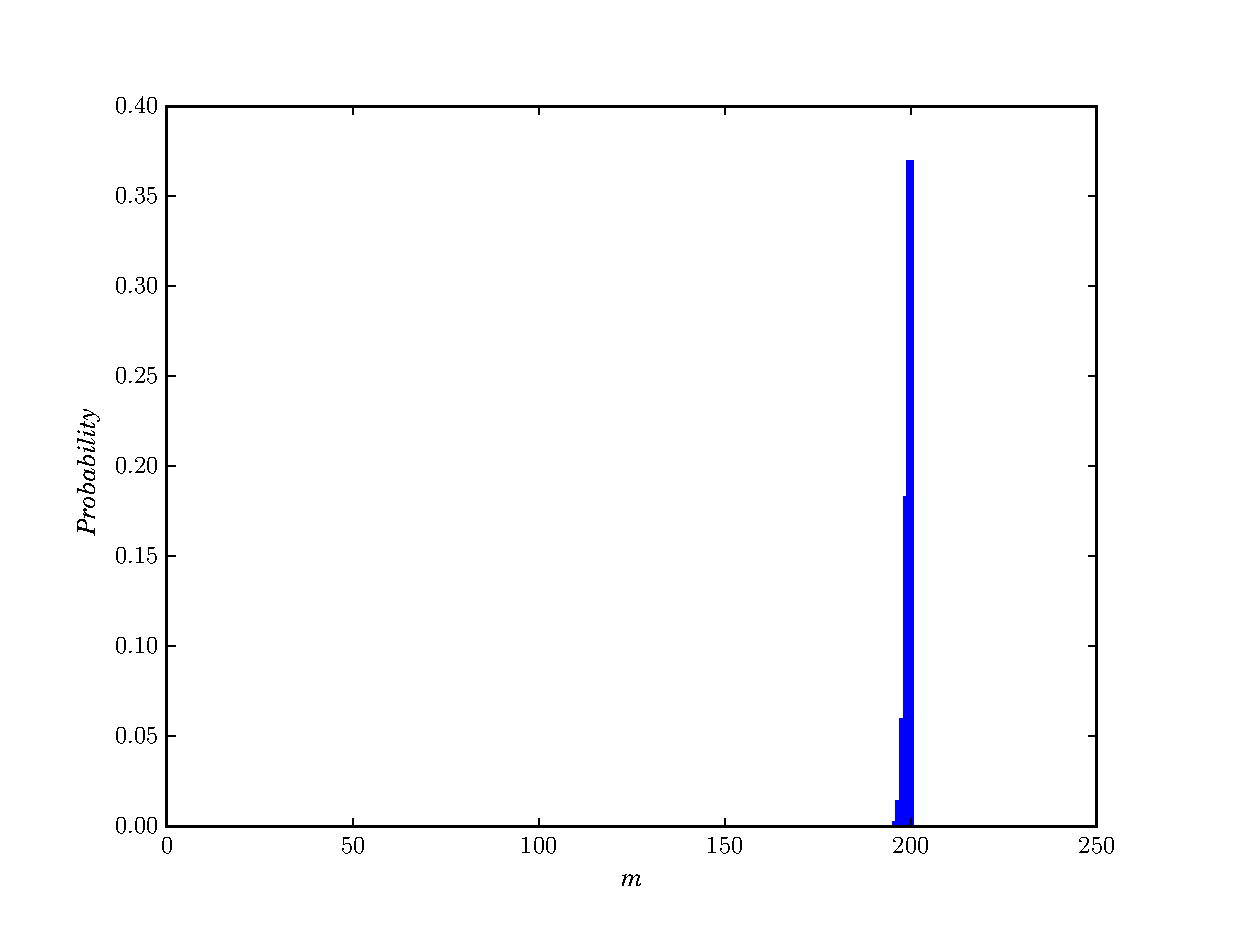
\includegraphics[scale=0.85]{../../plots/figure1}
	\caption{Probability distribution of having $m$ ancestors after $10000$ Moran generations for $n = 200$ in a constant haploid population size of $N = 20000$. We can see that there is a non-negligible amount of probability with losing more than a single lineage in this time. However, we should note that the rescaling of time in this case is quite important.}
\end{figure}
\end{center}



\end{document}
